% textwidth in cm: 13.69804cm

%%%%%%%%%%%%%%%%%%%%%%%%%%%%%%%%%%%%%%%%%%%%%%%%%%%%%%%%%%%%%%%%%%%%%%%%%%%%%%%%
%
% Template license:
% CC BY-NC-SA 3.0 (http://creativecommons.org/licenses/by-nc-sa/3.0/)
%
%%%%%%%%%%%%%%%%%%%%%%%%%%%%%%%%%%%%%%%%%%%%%%%%%%%%%%%%%%%%%%%%%%%%%%%%%%%%%%%%

% cant hojas: media = 30 a 40

%----------------------------------------------------------------------------------------
%	PACKAGES AND OTHER DOCUMENT CONFIGURATIONS
%----------------------------------------------------------------------------------------

\documentclass[
11pt, % The default document font size, options: 10pt, 11pt, 12pt
%oneside, % Two side (alternating margins) for binding by default, uncomment to switch to one side
%chapterinoneline,% Have the chapter title next to the number in one single line
spanish,
singlespacing, % Single line spacing, alternatives: onehalfspacing or doublespacing
%draft, % Uncomment to enable draft mode (no pictures, no links, overfull hboxes indicated)
%nolistspacing, % If the document is onehalfspacing or doublespacing, uncomment this to set spacing in lists to single
%liststotoc, % Uncomment to add the list of figures/tables/etc to the table of contents
%toctotoc, % Uncomment to add the main table of contents to the table of contents
parskip, % Uncomment to add space between paragraphs
%codirector, % Uncomment to add a codirector to the title page
headsepline, % Uncomment to get a line under the header
]{MastersDoctoralThesis} % The class file specifying the document structure



%----------------------------------------------------------------------------------------
%	INFORMACIÓN DE LA MEMORIA
%----------------------------------------------------------------------------------------

%    Dispositivo de captura para la red TCN en formaciones ferroviarias de Trenes Argentinos
%    Diseño y captura de la red TCN en formaciones ferroviarias de Trenes Argentinos
%    Desarrollo de dispositivo de captura para red TCN en formaciones ferroviarias de Trenes Argentinos
%    Dispositivo de captura de red TCN para formaciones ferroviarias de Trenes Argentinos
%    Implementación de dispositivo de captura para la red TCN en formaciones ferroviarias de Trenes Argentinos
\thesistitle{Dispositivo de captura para una red TCN}

% Nombre del posgrado, se usa en la carátula y se puede usar el cualquier lugar del documento con el comando \degreename
\posgrado{Carrera de Especialización en Sistemas Embebidos} 
%\posgrado{Carrera de Especialización en Internet de las Cosas} 
%\posgrado{Carrera de Especialización en Intelegencia Artificial}
%\posgrado{Maestría en Sistemas Embebidos} 
%\posgrado{Maestría en Internet de las cosas}

\author{Ing. Diego Essaya} % Tu nombre, se usa en la carátula y se puede usar el cualquier lugar del documento con el comando \authorname

\director{Dr. Ing. Pablo Gomez (FIUBA)} % El nombre del director, se usa en la carátula y se puede usar el cualquier lugar del documento con el comando \dirname

\juradoUNO{Nombre del jurado 1 (pertenencia)} % Nombre y pertenencia del un jurado se usa en la carátula y se puede usar el cualquier lugar del documento con el comando \jur1name
\juradoDOS{Nombre del jurado 2 (pertenencia)} % Nombre y pertenencia del un jurado se usa en la carátula y se puede usar el cualquier lugar del documento con el comando \jur2name
\juradoTRES{Nombre del jurado 3 (pertenencia)} % Nombre y pertenencia del un jurado se usa en la carátula y se puede usar el cualquier lugar del documento con el comando \jur3name

\ciudad{Ciudad Autónoma de Buenos Aires}

\fechaINICIO{septiembre de 2019}
\fechaFINAL{marzo de 2023}


\keywords{Sistemas embebidos, FIUBA} % Keywords for your thesis, print it elsewhere with \keywordnames

\newcommand\todo[1]{\textcolor{red}{#1}}

\usepackage[T1]{fontenc}
\usepackage{inconsolata}

\lstset{
  basicstyle=\small\ttfamily,
  breaklines=true,
}

\begin{document}

\definecolor{light-gray}{gray}{0.95}

\frontmatter % Use roman page numbering style (i, ii, iii, iv...) for the pre-content pages

\pagestyle{plain} % Default to the plain heading style until the thesis style is called for the body content


%----------------------------------------------------------------------------------------
%	RESUMEN - ABSTRACT 
%----------------------------------------------------------------------------------------

\begin{abstract}
\addchaptertocentry{\abstractname} % Add the abstract to the table of contents
%
%The Thesis Abstract is written here (and usually kept to just this page). The page is kept centered vertically so can expand into the blank space above the title too\ldots
\centering

La presente memoria describe el diseño y desarrollo de un dispositivo que permite capturar la información que circula por la red interna de una formación ferroviaria. Este trabajo fue desarrollado como parte de la convocatoria de Proyectos de Desarrollo Estratégico 2020 de UBACyT, con Trenes Argentinos como entidad adoptante.

El dispositivo desarrollado permite que Trenes Argentinos pueda monitorear los diferentes subsistemas presentes en una formación ferroviaria, ya sea para visualizar su estado en tiempo real o para archivar. Esto cubre la falta de tecnología propia para operar y mantener las formaciones, ya que históricamente hubo que recurrir a empresas extranjeras que ofrecen productos cerrados y de difícil acceso. En el trabajo se aplicaron conocimientos de protocolos de comunicación, programación de microprocesadores y programación de alto nivel.

\end{abstract}

%----------------------------------------------------------------------------------------
%	CONTENIDO DE LA MEMORIA  - AGRADECIMIENTOS
%----------------------------------------------------------------------------------------

\begin{acknowledgements}
\addchaptertocentry{\acknowledgementname}
\vspace{1.5cm}

A Pablo Gomez por su invaluable ayuda en la elaboración de este trabajo.

A los organizadores de la Carrera de Especialización en Sistemas Embebidos por otorgarme una beca, y brindarme la oportunidad de participar en el GICSAFe.

Al personal de la Gerencia de Material Rodante Eléctrico y del Laboratorio de Electrónica de Castelar de Trenes Argentinos por su colaboración y paciencia en la realización de las mediciones, en particular a Sergio Dieleke y Bruno Pilato.

\end{acknowledgements}

%----------------------------------------------------------------------------------------
%	LISTA DE CONTENIDOS/FIGURAS/TABLAS
%----------------------------------------------------------------------------------------

\tableofcontents % Prints the main table of contents

\listoffigures % Prints the list of figures

% \listoftables % Prints the list of tables


%----------------------------------------------------------------------------------------
%	CONTENIDO DE LA MEMORIA  - CAPÍTULOS
%----------------------------------------------------------------------------------------

\mainmatter % Begin numeric (1,2,3...) page numbering

\pagestyle{thesis} % Return the page headers back to the "thesis" style

% Incluir los capítulos como archivos separados desde la carpeta Chapters

\chapter{Introducción general}

En este capítulo se presenta el marco general del trabajo. Se detallan las motivaciones que llevaron a Trenes Argentinos a solicitar su desarrollo, y se realiza una revisión del estado del arte en cuanto a los productos comerciales disponibles. Se describe la propuesta inicial y las razones por las que posteriormente se decidió descartarla, y se exponen el alcance y los objetivos de la propuesta final.

\label{cap:IntroGeneral}

\section{Motivación}

La empresa Trenes Argentinos \cite{web:sofse} adquirió en 2013 un total de 705 unidades eléctricas múltiples (EMU) a la empresa china CRRC Qingdao Sifang \cite{web:sifang} \cite{licitacion1}. Estos vehículos prestan servicios en las líneas Mitre, Sarmiento y Roca desde 2014 \cite{emu:roca} \cite{emu:mitre-sarmiento}.

% TODO: la licitacion1 es para las lineas Sarmiento y Mitre. Falta la de Roca.
% TODO: esta bien citar wikipedia?

\begin{figure}[htbp]
	\centering
	\includegraphics[width=.5\textwidth]{./Figures/1082px-Línea_Mitre_Retiro.jpg}
	\caption[Unidad eléctrica múltiple (EMU)]{Una unidad eléctrica múltiple (EMU) en la estación Retiro de la línea Mitre, en Buenos Aires.\footnotemark}
	\label{fig:emu}
\end{figure}
\footnotetext{Fotografía por Casa Rosada (Argentina Presidencia de la Nación), CC BY-SA 2.0, \url{https://commons.wikimedia.org/w/index.php?curid=39117175}}

Los distintos subsistemas electrónicos presentes en una EMU (control de frenos, control de tracción, control de puertas, paneles de información al pasajero, etc.) están interconectados formando una red de datos. Mediante esta red, los componentes comparten datos de diagnóstico y reciben órdenes de control a distancia. La red interna que se utiliza en las EMU es una implementación del estándar TCN (Train Communication Network, IEC 61375-1 \cite{iec61375-1}).

Actualmente, Trenes Argentinos carece del conocimiento y las herramientas necesarias para interactuar con la red TCN en las EMU, de forma tal de poder capturar la información disponible, o agregar dispositivos de desarrollo propio.
Además, no dispone de un sistema de monitoreo a distancia que permita observar en tiempo real el estado de cada uno de los componentes de una formación ferroviaria.
Tampoco cuenta con un sistema de almacenamiento histórico del estado de los componentes, de forma tal de poder hacer pericia en caso de un accidente.

Estas limitaciones se vuelven más evidentes con frecuencia. Un ejemplo común es cuando una formación queda varada en un punto alejado de una estación, obligando a los técnicos a trasladarse personalmente para resolver el problema.
También es común la quema de fusibles, un inconveniente difícil de diagnosticar sin el monitoreo de variables como la tensión de línea.
Otro desafío adicional es la falta de control sobre las variables del sistema de aire acondicionado, lo que dificulta garantizar el confort y la seguridad de los pasajeros.


\section{Estado del arte}

La norma IEC 61375-1 es la fuente de información principal acerca del estándar TCN. Lamentablemente no hay mucha información adicional de libre acceso acerca del estándar, como artículos y notas de aplicación. Entre las publicaciones que citan a la norma tal vez las más relevantes son \textit{Design and implementation of MVB protocol analyzer} \cite{mvb-pub-1} (escrita en idioma chino) y \textit{An MVB signal capturer based on microcontrollers for metro train on-line health monitoring system} \cite{mvb-pub-2}, siendo ambas demasiado cortas como para aportar información realmente útil.

La mayoría de los equipos desarrollados hasta la fecha que funcionan de acuerdo al estándar TCN se basa en dos ASICs\footnote{Application-specific integrated circuit.} diferentes: el circuito MVBCS1 \cite{mvbcs1}, producido originalmente por la compañía ABB, aunque hoy en día es comercializado por Siemens, y el MVBC02C \cite{mvbc02c}, producido por Bombardier. Debido a su naturaleza, estos circuitos presentan características rígidas que no son apropiadas para satisfacer la amplia gama de posibilidades con respecto al tipo de nodos conectados a la red TCN \cite{mvb-pub-3}.

Otra publicación de interés es \textit{A Novel SoC Architecture for a MVB Slave Node} \cite{mvb-pub-3}, donde se describe el diseño de una arquitectura SoC\footnote{System on a chip.} compatible con el estándar TCN, basado en una FPGA\footnote{Field-programmable gate array.}.

Es posible encontrar en el mercado soluciones más intergadas, que podrían proporcionar una solución parcial a los problemas que afronta Trenes Argentinos. A continuación se presentan algunos de estos dispositivos, así como sus características principales.

\subsection{Yacer -- MVB-Analyzer}

El analizador de protocolo \textit{MVB-Analyzer} de la empresa Yacer \cite{yacer} proporciona una interfaz MVB, dos interfaces Ethernet y dos interfaces de expansión para recopilar y recibir tramas MVB y WTB, entre otras, y enviarlas a una computadora a través de una interfaz Ethernet. El producto incluye un software que permite analizar los datos del bus MVB y realizar simulaciones para encontrar la resolución de problemas y evaluar el funcionamiento del bus MVB.

\begin{figure}[htbp]
	\centering
	\includegraphics[height=20\baselineskip]{./Figures/yacer.jpg}
	\caption[Yacer -- MVB-Analyzer]{El analizador de protocolo \textit{MVB-Analyzer} de la empresa Yacer.}
\end{figure}

\subsection{AMiT Transportation -- WTB and MVB Analyzers}

Los analizadores del bus WTB y MVB de la empresa AMiT Transportation \cite{amit} son dispositivos de bus pasivos que monitorean el tráfico en la red y lo pasan al bus Ethernet en tramas UDP. Se conecta una PC al bus Ethernet con un programa para recibir y evaluar las tramas UDP.

El analizador solo monitorea el bus, y es "invisible" para otros dispositivos. Se monitorean todas las tramas WTB o MVB en el bus, que son transmitidas por el bus Ethernet a la PC. El producto incluye un complemento para el programa de código abierto Wireshark \cite{wireshark}, que permite analizar las tramas capturadas.

\begin{figure}[htbp]
	\centering
	\includegraphics[height=20\baselineskip]{./Figures/amit.jpg}
	\caption[AMiT Transportation -- WTB and MVB Analyzers]{El analizador de bus MVB de la empresa AMiT Transportation.}
\end{figure}


\subsection{Duagon -- D442 MVB Diagnostic System}

El sistema de diagnóstico MVB de la empresa Duagon \cite{duagon} está diseñado para depurar dispositivos y redes MVB. El sistema se conecta a una PC común, y puede funcionar en dos modos de operación:

\begin{itemize}
\item En el modo \emph{monitor}, el sistema permite investigar dispositivos MVB en el bus, leer y escribir la base de datos MVB, y escanear los puertos de los dispositivos, entre otras cosas.
\item En el modo \emph{servidor}, el sistema permite ejecutar aplicaciones programadas por el usuario. Se incluye una biblioteca de programación MVB con todas las funciones en el sistema de diagnóstico para controlar una red MVB completa.
\end{itemize}

\begin{figure}[htbp]
	\centering
	\includegraphics[width=0.5\textwidth]{./Figures/duagon.png}
	\caption[Duagon -- D442 MVB Diagnostic System]{El sistema de diagnóstico MVB de la empresa Duagon}
\end{figure}


\section{Propuesta inicial}

% En este contexto, Trenes Argentinos y el Grupo de Investigación en Calidad y Seguridad de las Aplicaciones Ferroviarias (GICSAFe) \cite{web:gicsafe} arman un grupo de trabajo para encontrar una solución.


\section{Alcance y objetivos}

\chapter{Introducción específica}

En este capítulo se presenta un resumen de los conceptos más relevantes acerca de la red TCN y su implementación en las formaciones de Trenes Argentinos, y se detallan las diferentes tecnologías utilizadas para el desarrollo del dispositivo de captura.

\section{La red TCN}

La red TCN es una combinación jerárquica de dos buses de datos para transmitir información dentro de una formación ferroviaria. El Multifunction Vehicle Bus (MVB) interconecta los diferentes dispositivos presentes dentro de cada vehículo, y el Wire Train Bus (WTB) interconecta los diferentes vehículos. Los componentes de la red TCN están estandarizados en la norma IEC 61375-1.

\begin{figure}[htbp]
	\centering
	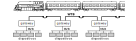
\includegraphics[width=.8\textwidth]{./Figures/tcn-mvb-wtb.png}
	\caption[Wire Train Bus y Multifunction Vehicle Bus]{Wire Train Bus y Multifunction Vehicle Bus.
        \\ \todo{CAMBIAR: La imagen original tiene copyright.}}
\end{figure}

Teniendo en cuenta que el dispositivo desarrollado se conecta al bus MVB, a continuación se exponen las características principales de este bus de comunicación.

\subsection{El bus MVB}

El MVB es el bus que interconecta diferentes dispositivos ubicados en el mismo vehículo o en diferentes vehículos. Proporciona tanto la interconexión de equipos programables entre sí como la interconexión de estos equipos con sus sensores y actuadores. El MVB puede direccionar hasta 4095 dispositivos, y puede reemplazar a WTB en formaciones en las que los vehículos no son separados durante su operación normal.

El MVB transporta tres tipos de información:

\begin{itemize}
\item \texttt{Process\_Data}: transmisión \textit{broadcast} periódica con dirección de origen, con un período de hasta 1 ms.
\item \texttt{Message\_Data}: transmisión bajo demanda, con dirección de destino \textit{unicast} o \textit{broadcast}.
\item \texttt{Supervisory\_Data}: datos intercambiados con el propósito de resolución de eventos, transferencia de control \textit{master} o transmisión de información de tipo \texttt{Device\_Status}.
\end{itemize}

\subsection{Capa física MVB}

El bus MVB ofrece tres opciones para la capa física:

\begin{itemize}
\item El medio Electrical Short Distance (ESD), para distancias de hasta 20 m, que soporta hasta 32 dispositivos por segmento, con transceptores de tipo RS-485.
\item El medio Electrical Middle Distance (EMD), para distancias de hasta 200 m, que soporta hasta  32 dispositivos por segmento, con transformadores y transceptores compatibles con la norma IEC 61158-2 \cite{iec61158_2}.
\item El medio Optical Glass Fibre (OGF), para distancias de hasta 2000 m, soportando conexiones punto a punto o subredes de topología tipo estrella.
\end{itemize}

En algunas formaciones el bus MVB puede abarcar varios vehículos, y un segmento EMD puede abarcar hasta 200 m, lo que equivale a unos 4 vehículos, sin repetidores. La norma recomienda este medio para conectar vehículos que se acoplan y desacoplan con frecuencia en la vía.

Las direcciones de los dispositivos se asignan durante la configuración de la red y no cambian durante la operación. Puede haber diferentes buses en un vehículo, interconectados mediante un \textit{gateway} al bus WTB.

\begin{figure}[htbp]
	\centering
	\includegraphics[width=1\textwidth]{./Figures/tcn-emd-esd-wtb.png}
	\caption[MVB abarcando tres vehículos]{MVB abarcando tres vehículos.
        \\ \todo{CAMBIAR: La imagen original tiene copyright.}}
\end{figure}

\subsection{Señalización MVB}

Todos los medios MVB operan a una velocidad unificada de 1,5 Mbit/s.

La información se transmite utilizando una codificación Manchester, que combina en una única señal la información y el \textit{clock}. Un ``1'' se transmite como una transición negativa en el medio de una celda de bit, y un ``0'' se transmite como una transición positiva.

\begin{figure}[htbp]
	\centering
	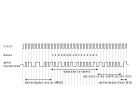
\includegraphics[width=1\textwidth]{./Figures/manchester.png}
	\caption[Delimitador de trama, información codificada con Manchester y la secuencia de verificación]{Delimitador de trama, información codificada con Manchester y la secuencia de verificación.
        \\ \todo{CAMBIAR: La imagen original tiene copyright.}}
\end{figure}

\subsection{Tramas MVB}

En el bus MVB se transmiten dos tipos de tramas:

\begin{itemize}
\item La trama \textit{master}, que es transmitida únicamente por el dispositivo maestro del bus.
\item La trama \textit{slave}, que es transmitida por un dispositivo esclavo en respuesta a una trama \textit{master}.
\end{itemize}

Ambos tipos de tramas son precedidas por un delimitador que marca el comienzo de la transmisión, y son sucedidas por una secuencia de verificación y un delimitador para marcar la finalización.

Una secuencia de una trama \textit{master} seguida de una trama \textit{slave} conforman un \textit{telegrama}.

\begin{figure}[htbp]
	\centering
	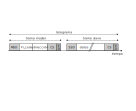
\includegraphics[width=1\textwidth]{./Figures/telegrama.png}
	\caption[Un telegrama MVB]{Un telegrama MVB.
        \\ \todo{CAMBIAR: La imagen original tiene copyright.}}
\end{figure}

Las tramas \textit{master} tienen una longitud fija de 16 bits (sin contar los delimitadores), e incluyen:

\begin{itemize}
\item Un código de 4 bits llamado \texttt{F\_code}, que indica el tipo y tamaño de la trama \textit{slave} esperada a continuación.
\item Un campo de 12 bits, que puede contener una dirección de destino, o parámetros específicos al \texttt{F\_code}.
\end{itemize}

Todos los dispositivos conectados al bus decodifican la trama \textit{master}. El dispositivo direccionado luego responde con su trama \textit{slave}, que a su vez puede ser recibida por otros dispositivos.

\section{TCN en Trenes Argentinos}

\section{Componentes del sistema}
 
\chapter{Diseño e implementación}
\label{cap:DisenioImplementacion}

En este capítulo se presenta la arquitectura de hardware y software del dispositivo de captura, como así también del generador de señal MVB desarrollado para probar el dispositivo de captura sin necesidad de conectarlo en una formación ferroviaria.

\section{Arquitectura de hardware}
\label{sec:hardware}

Como se muestra en la figura~\ref{fig:conexion}, el dispositivo de captura tiene dos conectores DE-9 compatibles con el medio EMD. De esta manera se lo puede conectar a un segmento MVB entre dos dispositivos cualesquiera.

\begin{figure}[htbp]
	\centering
    {
        \fontfamily{phv}
        \fontsize{8pt}{8pt}\selectfont
        \input{./Figures/conexion.pdf_tex}
    }
	\caption{Conexión del dispositivo de captura en un segmento EMD.}
    \label{fig:conexion}
\end{figure}

En la figura~\ref{fig:bloques} se muestra un diagrama de la arquitectura del dispositivo de captura.
Se dejan en corto circuito las líneas de transmisión (ver figura~\ref{fig:pines}), de forma tal de que el dispositivo opere en forma pasiva. Salvando la impedancia que agrega a la línea, el dispositivo de captura es transparente para el resto de los dispositivos del segmento.
El dispositivo MAX485 \cite{max485} se utiliza para convertir la señal de entrada (par diferencial $-$5~V - +5~V) a una señal compatible para el analizador lógico VKTECH (0~V - +5~V). El analizador lógico se conecta a una Raspberry Pi mediante un puerto USB 2.0. La Raspberry Pi decodifica las tramas por software y almacena los datos capturados en una tarjeta de memoria. Mediante su interfaz Wi-Fi se puede conectar una PC (utilizando el protocolo SSH) para descargar las capturas, y también para visualizar el tráfico del bus MVB en tiempo real.

\begin{figure}[htbp]
	\centering
    {
        \fontfamily{phv}
        \fontsize{8pt}{8pt}\selectfont
        \input{./Figures/bloques.pdf_tex}
    }
	\caption{Arquitectura de hardware del dispositivo de captura.}
    \label{fig:bloques}
\end{figure}

En la figura~\ref{fig:esquematico} se muestra un diagrama esquemático con el detalle de las conexiones entre los diferentes componentes. En el diagrama se utiliza la etiqueta ``USB'' para representar la conexión a la Raspberry Pi, que no se muestra por simplicidad. Asimismo, la conexión ``VCC'' del MAX485 se conecta al pin número 2 del conector GPIO de la Raspberry Pi \cite{gpio}.

\begin{figure}[htbp]
	\centering
	\includegraphics[width=1\textwidth]{./Figures/esquematico.png}
	\caption{Diagrama esquemático del dispositivo de captura.}
    \label{fig:esquematico}
\end{figure}

En la figura~\ref{fig:fotodispositivo} se muestra una foto del dispositivo de captura en construcción. Cabe aclarar que en el dispositivo hay cuatro MAX485 para permitir, en el futuro, capturar ambas líneas A y B del segmento EMD, o bien capturar dos o más segmentos diferentes. En esta primera versión del dispositivo se utiliza solo uno de los MAX485.

\begin{figure}[htbp]
	\centering
	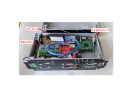
\includegraphics[width=1\textwidth]{./Figures/foto-dispositivo.pdf}
	\caption{Foto del dispositivo de captura en construcción.}
    \label{fig:fotodispositivo}
\end{figure}

\section{Arquitectura de software}
\label{sec:software}

Como se ve en la figura~\ref{fig:bloques}, la señal digital capturada por el VKTECH se envía a la Raspberry Pi en tiempo real mediante la interfaz USB. Para recibir esta señal en la Raspberry Pi se utiliza Sigrok, invocándolo de la siguiente manera:

\begin{lstlisting}[basicstyle=\small,breaklines=true]
$ sigrok-cli -d fx2lafw --continuous --config samplerate=12m
             --channels D0 -O binary
\end{lstlisting}

Los parámetros utilizados son:

\begin{itemize}
    \item \texttt{-d fx2lafw}: utilizar el \textit{driver} compatible con el dispositivo VKTECH.
    \item \texttt{--continuous}: muestrear en forma continua hasta ser detenido.
    \item \texttt{--config samplerate=12m}: muestrear con una frecuencia de 12 MHz.
    \item \texttt{--channels D0}: muestrear únicamente el canal 0 (correspondiente al pin \texttt{CH1} de la figura \ref{fig:esquematico}).
    \item \texttt{-O binary}: producir como salida un flujo de datos en formato binario.
\end{itemize}

Por cada muestra capturada, se emite un byte en el que cada bit corresponde a uno de los 8 canales del VKTECH.
Como se captura únicamente el canal 0, el bit menos significativo será 0 o 1 dependiendo de si la señal lógica capturada es baja o alta.
De esta forma, el flujo de datos tiene un ancho de banda de 12 MB/s, aunque se usa solo uno de los 8 bits de cada byte.
Este flujo de datos se puede redireccionar a un archivo o a un \textit{pipe} de Unix.

En la figura~\ref{fig:sigrok} se muestra un ejemplo del flujo de datos producido por Sigrok. El intervalo de 666,7 ns corresponde a un bit de datos de una trama MVB en codificación Manchester (ver figura~\ref{fig:manchester}). La frecuencia de muestreo de 12 MHz produce una muestra cada 83,33 ns.

\begin{figure}[htbp]
	\centering
    {
        \fontfamily{phv}
        \fontsize{9pt}{9pt}\selectfont
        \input{./Figures/sigrok.pdf_tex}
    }
	\caption{Flujo de datos producido por Sigrok.}
    \label{fig:sigrok}
\end{figure}

Sería posible bajar la frecuencia de muestreo, pero dado que la señal MVB se transmite a 1,5 Mbit/s en codificación Manchester, para lograr una captura suficientemente confiable el límite inferior es 6 MHz.
Sin embargo, la captura en una frecuencia cercana al límite inferior aumenta considerablemente la tasa de errores de captura.
La frecuencia elegida de 12 MHz ofrece un buen balance entre confiabilidad y eficiencia en espacio.

El flujo de datos producido por Sigrok se redirecciona mediante un \textit{pipe} de Unix a un software programado en lenguaje Go. Como se muestra en la figura~\ref{fig:capas-software}, la decodificación se realiza en tres capas de procesamiento:

\begin{enumerate}
\item La capa inferior (\texttt{MVBStream}) lee el flujo de datos byte por byte y ofrece funcionalidades tales como leer muestras individualmente, esperar hasta la siguiente transición de estado (alto-bajo o bajo-alto), esperar una cantidad de tiempo, etc.
\item La capa intermedia (\texttt{MVBDecoder}) identifica las tramas MVB y por cada telegrama produce un evento (\texttt{Event}).
\item La capa superior recibe los eventos y los procesa según el modo de operación del software. Se ofrecen dos modos de operación:
    \begin{itemize}
        \item En el modo interactivo, el software presenta una interfaz de usuario en la que se muestra el tráfico MVB en tiempo real.
        \item En el modo de almacenamiento, el software permite almacenar la evolución histórica de una o más variables de importancia.
    \end{itemize}
\end{enumerate}

\begin{figure}[htbp]
	\centering
    {
        \fontfamily{phv}
        \fontsize{9pt}{9pt}\selectfont
        \input{./Figures/capas-software.pdf_tex}
    }
	\caption{Capas de procesamiento del software de captura.}
    \label{fig:capas-software}
\end{figure}

En la figura~\ref{fig:interactivo} se muestra una captura de pantalla del modo interactivo.
En esta pantalla se presenta al usuario un resumen de la información capturada en tiempo real.
En la figura se destacan algunas secciones de la pantalla, que se detallan a continuación.

\begin{enumerate}
\item Total de telegramas capturados desde el inicio.
\item Cantidad de tiempo transcurrido desde el inicio.
\item Histograma de la cantidad de telegramas capturados en los últimos 10 segundos.
\item Tasa de telegramas capturados por segundo.
\item Histograma y tasa de telegramas por segundo, desglosado por el valor del \texttt{F\_code}.
\item Listado del último valor transmitido de cada variable, ordenado por puerto. El usuario puede elegir el rango de puertos a visualizar en esta lista.
\item Histograma y listado de los últimos errores de decodificación.
\end{enumerate}

\begin{figure}[htbp]
	\centering
	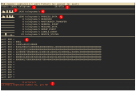
\includegraphics[width=1\textwidth]{./Figures/modo-interactivo.pdf}
	\caption{Modo interactivo del software de captura.}
    \label{fig:interactivo}
\end{figure}

En el modo de almacenamiento, el software se configura con un conjunto de variables a capturar, y almacena la evolución histórica de dichas variables.
Para el almacenamiento histórico se genera una carpeta por cada día de captura, y en cada carpeta un archivo CSV por cada variable capturada.

Por ejemplo, si se desea capturar los primeros 6 bytes del puerto \texttt{0x002} y el byte 8 del puerto \texttt{0x003}, se debe ejecutar el programa de la siguiente manera:

\begin{lstlisting}[basicstyle=\small,breaklines=true]
$ go run record/main.go 002:0:6 "fecha y hora" 003:8:9 "tension de red"
\end{lstlisting}

En la figura~\ref{fig:carpetas} se muestra la estructura de carpetas y archivos generada por el software al ser ejecutado con esta configuración.
Cada línea de los archivos CSV tiene el formato \texttt{<hora>,\allowbreak <valor>}, donde \texttt{<hora>} es la hora exacta en la que se transmitió la variable y \texttt{<valor>} es el valor de la variable.
Para conservar espacio, solo se agrega una línea al archivo CSV cuando la variable cambia de valor.

\begin{figure}[htbp]
	\centering
    {
        \ttfamily
        \fontsize{8pt}{8pt}\selectfont
        \input{./Figures/carpetas.pdf_tex}
    }
	\caption{Ejemplo de estructura de carpetas y archivos generado por el software en modo de almacenamiento.}
    \label{fig:carpetas}
\end{figure}

El software de captura se ejecuta en la Raspberry Pi que forma parte del dispositivo de captura.
Entre otras razones, se eligió el lenguaje Go porque permite compilar para Raspberry Pi con el siguiente comando:

\begin{lstlisting}[basicstyle=\small,breaklines=true,columns=fullflexible]
$ GOOS=linux GOARCH=arm GOARM=5 go build ./main.go
\end{lstlisting}

El código fuente del software de captura está disponible en la plataforma Github \cite{mvbparse-go}.
En el archivo \texttt{README.md} se muestran más detalles acerca de los diferentes modos de funcionamiento.

\section{Generador de señal de prueba MVB}
\label{sec:generador}

Para probar el funcionamiento del software de captura sin necesidad de acudir a un taller de Trenes Argentinos y conectar el dispositivo en una formación ferroviaria, se decidió desarrollar un dispositivo auxiliar. Este dispositivo genera una señal con características similares a la señal transmitida en el bus MVB, emitiendo una secuencia de tramas en forma cíclica.

En la figura~\ref{fig:generador} se muestra un diagrama de bloques con el generador de señal MVB conectado al VKTECH. La señal es generada por software en una EDU-CIAA, y se transmite mediante la interfaz SPI. La señal generada es similar a la señal producida por el MAX485 en la figura~\ref{fig:bloques}.

\begin{figure}[htbp]
	\centering
    {
        \fontfamily{phv}
        \fontsize{8pt}{8pt}\selectfont
        \input{./Figures/generador.pdf_tex}
    }
	\caption{Generador de señal MVB.}
    \label{fig:generador}
\end{figure}

El firmware desarrollado para el generador de señal está disponible en la plataforma Github \cite{mvbgen}.

Para simular el tráfico del bus, el firmware transmite un telegrama cada 750 microsegundos.
Los telegramas transmitidos son reproducciones de capturas realizadas en un bus MVB real (ver sección \ref{sec:capturas}). Por ejemplo, en el código~\ref{cod:telegrama} se muestra la definición del primer telegrama transmitido.
Los primeros 3 bytes corresponden a la trama \textit{master} (16 bits de datos más la secuencia de verificación) y a continuación se especifica el contenido de la trama \textit{slave}, de 36 bytes de longitud.

\begin{lstlisting}[label=cod:telegrama,caption=Definición de un telegrama a transmitir (\texttt{gen.c}).,float,numberstyle=\footnotesize\ttfamily,language=C,breaklines=true,numbers=left,firstnumber=11,xleftmargin=1cm]
static const telegram_t mvb_data[] = {
    { { 0x43, 0x90, 0xd6 }, (uint8_t[]){ 0x97, 0x1e, 0x00, 0x00, 0x00, 0x82, 0x14, 0x06, 0xdf, 0x1e, 0x0b, 0x31, 0x0f, 0x00, 0x17, 0x05, 0x8c, 0xf8, 0x00, 0x00, 0x00, 0x00, 0x00, 0x00, 0x03, 0x4d, 0xc9, 0x11, 0x94, 0x11, 0xa8, 0x11, 0xa8, 0x04, 0x05, 0x88 }, 36 },
\end{lstlisting}

Para enviar un telegrama, se envía la trama \textit{master}, luego se transmiten 15 bits en alto (esto simula una pequeña pausa entre las tramas), y luego se transmite la trama \textit{slave}. Esta secuencia de pasos se muestra en el código~\ref{cod:send}.

\begin{lstlisting}[label=cod:send,caption=Secuencia de pasos para transmitir un telegrama (\texttt{gen.c}).,float,numberstyle=\footnotesize\ttfamily,language=C,breaklines=true,numbers=left,firstnumber=193,xleftmargin=1cm]
    send_master(mvb_data[i].master);
    send_idle(15, 1);
    send_slave(mvb_data[i].slave, mvb_data[i].slave_len);
\end{lstlisting}

Como se muestra en el código~\ref{cod:sendmaster}, para transmitir la trama \textit{master}, se envía el delimitador inicial, seguido de los 3 bytes de la trama y el delimitador final. La transmisión de la trama \textit{slave} es similar.

\begin{lstlisting}[label=cod:sendmaster,caption=Secuencia de pasos para transmitir la trama \textit{master} (\texttt{gen.c}).,float,numberstyle=\footnotesize\ttfamily,language=C,breaklines=true,numbers=left,firstnumber=173,xleftmargin=1cm]
static void send_master(const uint8_t bytes[]) {
    send_start_bit();
    send_master_start_delimiter();
    send_bytes(bytes, 3);
    send_end_delimiter();
}
\end{lstlisting}

Las funciones previamente mencionadas cargan la información a transmitir en un \textit{buffer}. Cada bit de información se codifica en Manchester: un bit ``1'' corresponde a una transición negativa y se traduce en dos bits 1-0, y un bit ``0'' corresponde a una transición positiva y se traduce en dos bits 0-1. De esta manera, cada bit de información que se carga ocupa 2 bits en el \textit{buffer}.

En el código~\ref{cod:main} se muestra el ciclo principal del programa, en el que se hace una pausa de 750 microsegundos, luego se prepara el siguiente telegrama a transmitir en el \textit{buffer}, y luego se transmite el contenido del \textit{buffer} mediante la interfaz SPI.

\begin{lstlisting}[label=cod:main,caption=Ciclo principal del programa (\texttt{main.c}).,float,numberstyle=\footnotesize\ttfamily,language=C,breaklines=true,numbers=left,firstnumber=31,xleftmargin=1cm]
    while (1) {
        delayInaccurateUs(750);
        sendbuf_t *buf = next_telegram();
        spiWrite(SPI0, buf->data, buf->bytes);
    }
\end{lstlisting}

La interfaz SPI se configura para transmitir con una frecuencia de 3 Mbit/s, de forma tal que cada par de bits transmitidos corresponden a un bit de información codificada en Manchester. De esta manera se logra una tasa de 1,5 Mbit/s compatible con el protocolo MVB.

\chapter{Ensayos y resultados}

\label{cap:EnsayosResultados}

En este capítulo se describe la fase de investigación previa al desarrollo del dispositivo de captura, junto con las pruebas realizadas para validar su correcto funcionamiento, tanto en un entorno de laboratorio como en una formación de Trenes Argentinos.

\section{Capturas del tráfico de la red en una formación}
\label{sec:capturas}

Como parte de la etapa de investigación, se realizó en junio de 2020 una visita al taller Victoria de Trenes Argentinos, coordinada por Sergio Dieleke (Coordinador Laboratorio Electrónico, Subgerencia de Material Rodante Línea Mitre). El objetivo principal de la visita fue tomar capturas del tráfico del bus MVB, para tomar conocimiento acerca del estándar TCN y de la implementación particular en las EMU de Trenes Argentinos.

Para tomar las capturas se conectó un MAX485 y un analizador lógico VKTECH entre dos dispositivos MVB.
También se utilizó un osciloscopio para verificar que la señal capturada tuviera las características esperadas.
En la figura~\ref{fig:banco-capturas} se muestra un diagrama de bloques del banco de medición.
En las figuras~\ref{fig:foto-banco-capturas} y \ref{fig:osciloscopio} se muestra una fotografía del banco de medición y un detalle de la señal capturada en el osciloscopio.

% video con la secuencia https://drive.google.com/drive/folders/1I-V33ElLX13Iy0YliUeojRwYFQKuucAO
\begin{figure}[htbp]
	\centering
    {
        \fontfamily{phv}
        \fontsize{9pt}{9pt}\selectfont
        \input{./Figures/banco-captura.pdf_tex}
    }
	\caption{Banco de medición utilizado para tomar las capturas.}
    \label{fig:banco-capturas}
\end{figure}

\begin{figure}[htbp]
	\centering
	\includegraphics[width=\textwidth]{./Figures/foto-capturas.jpg}
	\caption{Fotografía del banco de medición utilizado para tomar las capturas.}
    \label{fig:foto-banco-capturas}
\end{figure}

\begin{figure}[htbp]
	\centering
	\includegraphics[width=\textwidth]{./Figures/osciloscopio.jpg}
	\caption{Señal MVB capturada en el osciloscopio.}
    \label{fig:osciloscopio}
\end{figure}

Mediante la PC conectada con el analizador lógico se tomaron capturas de un minuto de duración del tráfico del bus MVB, con el banco de medición conectado en diferentes puntos del segmento.
En simultáneo con las capturas se efectuó el procedimiento de encendido de la red y una secuencia de pasos tales como tomar cabina, abrir y cerrar puertas, cambio de marcha, etc., de forma tal de generar tráfico en la red y así poder analizar en detalle el funcionamiento de la misma.

En la figura~\ref{fig:pulseview} se muestra una visualización de una de las capturas.
En la figura~\ref{fig:pulseview-10ms} se observa que en los primeros 10ms se transmitieron 10 telegramas, aunque en el nivel de detalle no es suficiente para discernir su formato.
En la figura~\ref{fig:pulseview-telegrama} se amplía la visualización de uno de los telegramas, donde se puede apreciar en detalle las tramas \textit{master} y \textit{slave}.
Estas visualizaciones se obtuvieron utilizando el software PulseView, que es parte del proyecto Sigrok.

\begin{figure}[htbp!]
	\centering
    \begin{subfigure}[b]{\textwidth}
        \centering
        \includegraphics[width=\textwidth]{./Figures/pulseview-10ms.png}
        \caption{Algunos telegramas transmitidos en el transcurso de 10 ms.}
        \label{fig:pulseview-10ms}
    \end{subfigure}
    \par\bigskip
    \begin{subfigure}[b]{\textwidth}
        \centering
        \includegraphics[width=1\textwidth]{./Figures/pulseview-telegrama.png}
        \caption{Ampliación de un telegrama.}
        \label{fig:pulseview-telegrama}
    \end{subfigure}
    \caption{Visualización de una de las capturas realizadas.}
    \label{fig:pulseview}
\end{figure}

\section{Decodificación de las capturas}
\label{sec:decodificacion}

\section{Pruebas con el generador de señal}
\section{Captura en tiempo real}
 
\chapter{Conclusiones}

\label{cap:Conclusiones}

\section{Resultados obtenidos}
\section{Trabajo futuro}

% terminador EMD

% ESD

% WTB

% message data

% ethernet
 

%----------------------------------------------------------------------------------------
%	CONTENIDO DE LA MEMORIA  - APÉNDICES
%----------------------------------------------------------------------------------------

\appendix % indicativo para indicarle a LaTeX los siguientes "capítulos" son apéndices

% Incluir los apéndices de la memoria como archivos separadas desde la carpeta Appendices
% Descomentar las líneas a medida que se escriben los apéndices

%\include{Appendices/AppendixA}
%\include{Appendices/AppendixB}
%\include{Appendices/AppendixC}

%----------------------------------------------------------------------------------------
%	BIBLIOGRAPHY
%----------------------------------------------------------------------------------------

\Urlmuskip=0mu plus 1mu\relax
\raggedright
\printbibliography[heading=bibintoc]

%----------------------------------------------------------------------------------------

\end{document}  
